\section{Casos de Uso del Administrador}

\subsection{Diagrama de Casos de Uso General del Administrador}

\begin{figure}[htbp]
	\centering
		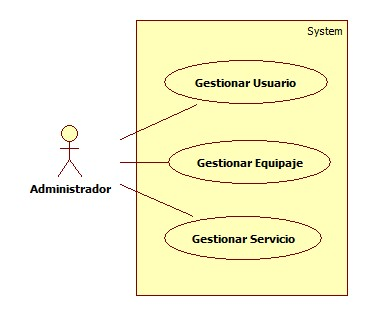
\includegraphics[width=0.4\textwidth]{Figuras/general.jpg}
		\rule{30em}{0.5pt}
	\caption[Diagrama de Casos de Uso General del Administrador]{Diagrama de Casos de Uso General del Administrador}
	\label{fig:cuGeneralAdministrador}
\end{figure}

\subsection{Caso de Uso Gestionar Usuario}

\begin{figure}[htbp]
	\centering
		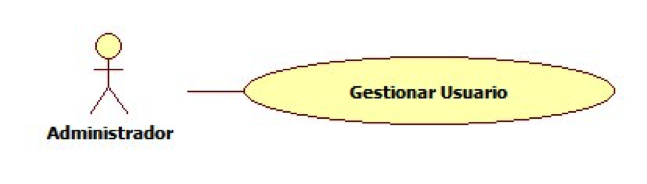
\includegraphics[width=0.9\textwidth]{Figuras/cuGestionarUsuario.png}
		\rule{30em}{0.5pt}
	\caption[Diagrama de Caso de Uso Gestionar Usuario]{Diagrama de Caso de Uso Gestionar Usuario}
	\label{fig:cuGestionarUsuario}
\end{figure}
\clearpage

\begin{longtable}{|p{2.5cm}|p{6.4cm}|p{2cm}|p{2cm}|}
	\hline
		\rowcolor[RGB]{51,153,255}{Caso de Uso}&\multicolumn{2}{c}{Gestionar Usuario}&{\textbf{CU-A-01}}\\
	\hline
		{Actores}&\multicolumn{3}{p{11.2cm}|}{Administrador}\\
	\hline
		{Tipo}&\multicolumn{3}{p{11.2cm}|}{Esencial}\\
	\hline
		{Precondición}&\multicolumn{3}{p{11.2cm}|}{El administrador se autentifica en el sistema.}\\
	\hline
		{Postcondición}&\multicolumn{3}{p{11.2cm}|}{Haber eliminado usuarios inactivos del sistema.}\\
	\hline
		{Autor}&{Vivanco Carmona Erick Rafael}&{\textbf{Fecha} 09/01/15}&{\textbf{Versión} 2.0}\\
			\hline
		{Evaluador}&{Barajas Uribe Sergio}&{\textbf{Fecha} 15/01/15}&{\textbf{Estatus} Aprobado}\\
	\hline
		{Propósito}&\multicolumn{3}{p{11.2cm}|}{Eliminar usuarios del sistema que hayan estado inactivos por mucho tiempo, de esta manera se tendrá un mayor control del número de usuarios del sistema.}\\
	\hline
		{Resumen}&\multicolumn{3}{p{11.2cm}|}{El administrador identifica usuarios inactivos y los da de baja.}\\	
	\hline
	\caption[Especificación del Caso de Uso Gestionar Usuario]{Especificación del Caso de Uso Gestionar Usuario}
    	\label{tab:cuGestionarUsuario}
\end{longtable}

\begin{flushleft}
	\textbf{Trayectoria Principal}\\
	\begin{enumerate}
		\item El administrador solicita la lista de usuarios.
		\item El sistema despliega los usuarios.
		\item El administrador identifica usuarios inactivos y los da de baja.
	\end{enumerate}
\end{flushleft}
----Fin del caso de uso
\clearpage

\subsection{Caso de Uso Gestionar Equipaje}

\begin{figure}[htbp]
	\centering
		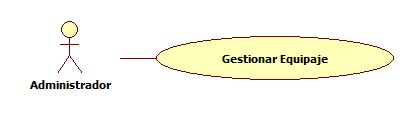
\includegraphics[width=0.9\textwidth]{Figuras/cuGestionarEquipaje.jpg}
		\rule{30em}{0.5pt}
	\caption[Diagrama de Caso de Uso Gestionar Equipaje]{Diagrama de Caso de Uso Gestionar Equipaje}
	\label{fig:cuGestionarEquipaje}
\end{figure}

\begin{longtable}{|p{2.5cm}|p{6.4cm}|p{2cm}|p{2cm}|}
	\hline
		\rowcolor[RGB]{51,153,255}{Caso de Uso}&\multicolumn{2}{c}{Gestionar Equipaje}&{\textbf{CU-A-02}}\\
	\hline
		{Actores}&\multicolumn{3}{p{11.2cm}|}{Administrador}\\
	\hline
		{Tipo}&\multicolumn{3}{p{11.2cm}|}{Esencial}\\
	\hline
		{Precondición}&\multicolumn{3}{p{11.2cm}|}{El administrador se autentifica en el sistema.}\\
	\hline
		{Postcondición}&\multicolumn{3}{p{11.2cm}|}{Registrar objetos para equipaje.}\\
	\hline
		{Autor}&{Vivanco Carmona Erick Rafael}&{\textbf{Fecha} 09/01/15}&{\textbf{Versión} 2.0}\\
			\hline
		{Evaluador}&{Barajas Uribe Sergio}&{\textbf{Fecha} 15/01/15}&{\textbf{Estatus} Aprobado}\\
	\hline
		{Propósito}&\multicolumn{3}{p{11.2cm}|}{Registrar objetos útiles para un equipaje de viaje.}\\
	\hline
		{Resumen}&\multicolumn{3}{p{11.2cm}|}{El administrador registra y elimina objetos que puedan ser útiles para el usuario al momento de generar un equipaje para su viaje.}\\	
	\hline
	\caption[Especificación del Caso de Uso Gestionar Equipaje]{Especificación del Caso de Uso Gestionar Equipaje}
    	\label{tab:cuGestionarEquipaje}
\end{longtable}

\begin{flushleft}
	\textbf{Trayectoria Principal}\\
	\begin{enumerate}
		\item El administrador solicita registrar equipaje.
		\item El administrador registra objetos. \hyperlink{TrayectoriaA_CU-A-02}{[Trayectoria A]}.
		\item Los objetos quedan disponibles para futuras listas de equipaje que el usuario desee crear.
		\item El administrador elimina objetos.
	\end{enumerate}
\end{flushleft}
----Fin del caso de uso

\begin{flushleft}
	\hypertarget{TrayectoriaA_CU-A-02}{}
	\textbf{Trayectoria Alternativa A}\\
	\textbf{Condición:} El administrador ha registrado un objeto. \\
	\begin{enumerate}
		\item El objeto ha sido creado y se notifica al administrador. 
		\item Volver a 2.
	\end{enumerate}
\end{flushleft}
----Fin de Trayectoria
\clearpage

\subsection{Caso de Uso Gestionar Servicio}

\begin{figure}[htbp]
	\centering
		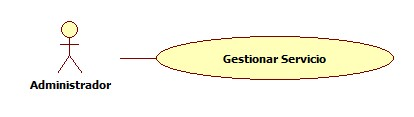
\includegraphics[width=0.9\textwidth]{Figuras/GestionarServicio.jpg}
		\rule{30em}{0.5pt}
	\caption[Diagrama de Caso de Uso Gestionar Servicio]{Diagrama de Caso de Uso Gestionar Servicio}
	\label{fig:cuGestionarServicio}
\end{figure}

\begin{longtable}{|p{2.5cm}|p{6.4cm}|p{2cm}|p{2cm}|}
	\hline
		\rowcolor[RGB]{51,153,255}{Caso de Uso}&\multicolumn{2}{c}{Gestionar Servicio}&{\textbf{CU-A-03}}\\
	\hline
		{Actores}&\multicolumn{3}{p{11.2cm}|}{Administrador}\\
	\hline
		{Tipo}&\multicolumn{3}{p{11.2cm}|}{Esencial}\\
	\hline
		{Precondición}&\multicolumn{3}{p{11.2cm}|}{El administrador se autentifica en el sistema.}\\
	\hline
		{Postcondición}&\multicolumn{3}{p{11.2cm}|}{Registrar servicios en el sistema.}\\
	\hline
		{Autor}&{Vivanco Carmona Erick Rafael}&{\textbf{Fecha} 09/01/15}&{\textbf{Versión} 2.0}\\
			\hline
		{Evaluador}&{Barajas Uribe Sergio}&{\textbf{Fecha} 15/01/15}&{\textbf{Estatus} Aprobado}\\
	\hline
		{Propósito}&\multicolumn{3}{p{11.2cm}|}{Registrar servicios del AICM para que el usuario pueda visualizarlos en su localización dentro del AICM.}\\
	\hline
		{Resumen}&\multicolumn{3}{p{11.2cm}|}{El administrador registra servicios del AICM.}\\	
	\hline
	\caption[Especificación del Caso de Uso Gestionar Servicio]{Especificación del Caso de Uso Gestionar Servicio}
    	\label{tab:cuGestionarServicio}
\end{longtable}

\begin{flushleft}
	\textbf{Trayectoria Principal}\\
	\begin{enumerate}
		\item El administrador desea gestionar servicios en el AICM.
		\item El administrador da de alta un servicio en una determinada coordenada en el AICM.
		\item El servicio queda registrado en el sistema, para posterior uso en la localización del usuario dentro del AICM.
		\item El administrador da de baja un servicio del AICM.
	\end{enumerate}
\end{flushleft}
----Fin del caso de uso
\clearpage